\documentclass[11pt, letterpaper]{article}
\usepackage{palatino}
\usepackage{graphicx}
\usepackage{enumitem}
\usepackage[top=1in, left=1in, right=1in, bottom=1in]{geometry}

\begin{document}
\begin{center}
\Large{\textbf{Capstone 2 - Model Metrics}}

\large{Kirsten Regier}
\end{center}

\section{Decision Tree Model}
\subsection{Hyperparameters}
The hyperparameters for depth and node purity method were determined by a grid search, as shown in Figure \ref{fig:DTHyper}. The optimal depth is 22 and node purity method is gini.

\begin{figure}[h]
\begin{center}
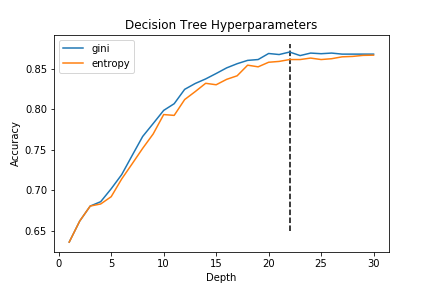
\includegraphics[width=3in]{DTHyperparameters.png}
\caption{Grid search results for \textbf{depth} and \textbf{node purity} method hyperparameters.} 
\label{fig:DTHyper}
\end{center}
\end{figure}

\subsection{Model parameters}
\noindent \textbf{DecisionTreeClassifier}(ccp\textunderscore alpha=0.0, class\textunderscore weight=None, criterion='gini', 
max\textunderscore depth=22, \newline 
max\textunderscore features=None, 
max\textunderscore leaf\textunderscore nodes=None, 
min\textunderscore impurity\textunderscore decrease=0.0, 
min\textunderscore impurity\textunderscore split=None, 
min\textunderscore samples\textunderscore leaf=1, 
min\textunderscore samples\textunderscore split=2, 
min\textunderscore weight\textunderscore fraction\textunderscore leaf=0.0, presort='deprecated', random\textunderscore state=21, splitter='best')

\begin{figure}[h]
\begin{center}
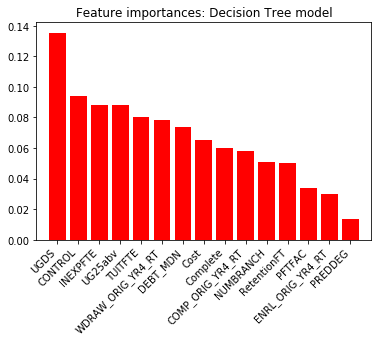
\includegraphics[width=2.5in]{DTFeatureImportance.png}
\caption{Feature importance levels based on the Decision Tree model.} 
\label{fig:DTFeatures}
\end{center}
\end{figure}

\subsection{Model evaluation}

\begin{table}[h]
\begin{center}
\caption{Decision Tree - Confusion matrix and Evaluation metrics}
\begin{tabular}{l l | c c r }
\multicolumn{2}{l}{Currently operating} & \multicolumn{2}{c}{Predicted} & Recall \\
& & No & Yes &  \\ 
\cline{2-5}
Actual & No & 1533 &  123 & 0.93 \\
& Yes & 380 & 1852 & 0.86 \\  \hline
Precision&  & 0.80 & 0.94 \\ 
Accuracy & & &  & 0.87 \\
\end{tabular}
\label{tab:DTConfusion}
\end{center}
\end{table} 

\section{AdaBoost Model}

\subsection{Hyperparameters}
The hyperparameter for number of estimators was determined by a grid search using the previous Decision Tree model as a base (orange) and without providing a base model (blue), as shown in Figure \ref{fig:ABHyper}. The optimal number of estimators is 122.

\begin{figure}[h]
\begin{center}
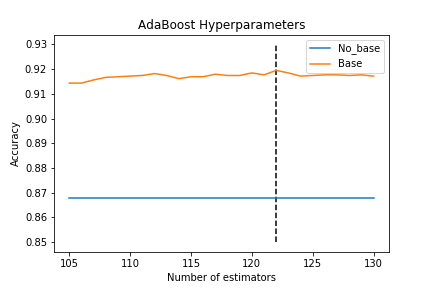
\includegraphics[width=3in]{ABHyperparameters.png}
\caption{Grid search results for \textbf{number of estimators} hyperparameter.} 
\label{fig:ABHyper}
\end{center}
\end{figure}

\subsection{Model parameters}
\noindent \textbf{AdaBoostClassifier}(algorithm='SAMME.R',
                   base\textunderscore estimator=DecisionTreeClassifier(ccp\textunderscore alpha=0.0,
                                                         class\textunderscore weight=None,
                                                         criterion='gini',
                                                         max\textunderscore depth=22,
                                                         max\textunderscore features=None,
                                                         max\textunderscore leaf\textunderscore nodes=None,
                                                         min\textunderscore impurity\textunderscore decrease=0.0,
                                                         min\textunderscore impurity\textunderscore split=None,
                                                         min\textunderscore samples\textunderscore leaf=1,
                                                         min\textunderscore samples\textunderscore split=2,
                                                         min\textunderscore weight\textunderscore fraction\textunderscore leaf=0.0,
                                                         presort='deprecated',
                                                         random\textunderscore state=21,
                                                         splitter='best'),
                   learning\textunderscore rate=1.0, n\textunderscore estimators=122, random\textunderscore state=21)

\begin{figure}[h]
\begin{center}
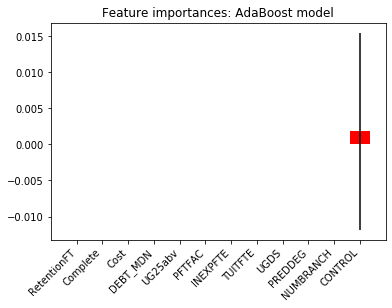
\includegraphics[width=3in]{ABFeatureImportance.png}
\caption{Feature importance levels based on the AdaBoost model.} 
\label{fig:Features}
\end{center}
\end{figure}

\newpage
\subsection{Model evaluation}

\begin{table}[h!]
 	\caption{AdaBoost model - Confusion matrices and Evaluation metrics} 
 	\begin{minipage}{.5\linewidth}
		\caption{Resampled data}
		\centering
		\begin{tabular}{l l | c c r }
\multicolumn{2}{l}{Currently operating} & \multicolumn{2}{c}{Predicted} & Recall \\
& & No & Yes &  \\ 
\cline{2-5}
Actual & No & 1538 & 118 & 0.93 \\
& Yes & 195 & 2037 & 0.91 \\  \hline
Precision&  & 0.89 & 0.95 \\ 
Accuracy & & &  & 0.92 \\
	\end{tabular}
	\label{tab:ABConfusionResamp}
	\end{minipage}%
	\begin{minipage}{.5\linewidth}
	\caption{Without duplicate data}
	\centering
		\begin{tabular}{l l | c c r }
\multicolumn{2}{l}{Currently operating} & \multicolumn{2}{c}{Predicted} & Recall \\
& & No & Yes &  \\ 
\cline{2-5}
Actual & No & 1164 &  93 & 0.93 \\
& Yes & 195 & 2037 & .91 \\  \hline
Precision&  & .86 & .96 \\ 
Accuracy & & &  & .92 \\
	\end{tabular}
	\label{tab:ABConfusionNoDup}	
	\end{minipage}
\end{table} 

\subsection{Threshold calculation}

Various thresholds for assigning schools to currently operating or not were tried for both the final Decision Tree model and the final AdaBoost model, as shown in Figure \ref{fig:Thresholds}. Initial models on the unbalanced dataset and the Decision Tree model showed that adjusting the threshold could improve model performance. However, after resampling the minority class to balance the data, and the using the AdaBoost model which focusses on misclassified data, improved the model performance to the point where the 50\% threshold produced the best scores for both accuracy and balanced accuracy.

\begin{figure}[h]
\begin{center}
\includegraphics[width=3in]{DTThreshold.png}
\includegraphics[width=3in]{ABThreshold.png}
\caption{Accuracy and balanced accuracy scores at various decision thresholds for the Decision Tree model (left) and AdaBoost model (right).} 
\label{fig:Thresholds}
\end{center}
\end{figure}

\end{document}